\chapter{Аналитическая часть}

\section{Одежда, как объект физического мира}

Любая одежда: футболки, брюки, носки, шарфы и куртки и т.~д., --- представляeт
собой одну или несколько соединенных между собой деталей из ткани. Ткань, в
свою очередь, состоит из натуральных или искусственных волокон или нитей,
которые производятся путем прядения различных материалов (рисунок \ref{fig:fibers}),
таких как шерсть, хлопок, лен~и~т.~п.
Для соединения полученных волокон используют следующие техники:
\begin{itemize}[left=\parindent]
    \item ткачество --- изготовление ткани путем переплетения нитей под прямым
        углом (рисунок \ref{subimg:wrap});
    \item вязание --- соедение волокон между собой путем образования и
        протягивания петель (рисунок \ref{subimg:knit});
    \item макраме --- закрепление нитей с помощью узлов (рисунок \ref{subimg:makrame});
    \item прессование волокон животных (получение войлока) (рисунок \ref{subimg:felt}).
\end{itemize}
После применения одной из этих техник получается готовая ткань.

~\\
\begin{figure}[ht!]
    \vspace{-4ex}
    \centering
    \subimg{25mm}{img00.jpg}{wool}
    \hspace{4ex}
    \subimg{25mm}{img01.jpg}{cotton}
    \hspace{4ex}
    \subimg{25mm}{img02.jpg}{linen}
    \caption{Виды волокон: 
             \subref{subimg:wool} шерсть,
             \subref{subimg:cotton} хлопок,
             \subref{subimg:linen} лен}
    \label{fig:fibers}
\end{figure}

\begin{figure}[ht!]
    \vspace{-4ex}
    \centering
    \subimg{50mm}{img03.jpg}{wrap}
    \hspace{4ex}
    \subimg{50mm}{img04.jpg}{knit}
    \vfill
    \hspace{4ex}
    \subimg{50mm}{img05.jpg}{makrame}
    \hspace{4ex}
    \subimg{50mm}{img06.jpg}{felt}
    \caption{Техники соединения волокон:
             \subref{subimg:wrap} ткачество,
             \subref{subimg:knit} вязание,~\\
             \subref{subimg:makrame} макраме,
             \subref{subimg:felt} войлок
            }
    \label{fig:getCloth}
\end{figure}

Разные волоконные материалы и техники их соединения являются причиной
различной степени проявления разными тканями основных механических свойств:
растяжения, сдвига и изгиба. Отсутвие у тканных материалов упругих
свойств приводит к образованию складок и легком драпировании на другие
объекты. Таким образом, разное строение ткани в зависимости от типа волокон,
большое количество узлов, из которых она состоит, разные
степени проявления механических свойств, большое количество степеней свободы -- все это
создает сложности при моделировании ткани. Поэтому существуют и разрабатываются
методы визуализации ткани, отвечающие различным требованиям: одни работают
быстро, но получаемые ими изображения менее реалистичны, другие создают
реалистичное изображение, что требуют бóльших затрат по времени. Поэтому
при решении задачи визуализации ткани часто приходится делать выбор
между скоростью и реалистичностью \cite{bib11}.

\section{Методы визуализации одежды}

Как уже было сказано выше, одежда является более сложной формой ткани,
поэтому далее будут рассмотрены методы моделирования тканных материалов.
Данные методы можно разделить на два основных типа:
\begin{itemize}[left=\parindent]
    \item геометрические методы;
    \item физические методы.
\end{itemize}

\subsection{Геометрические методы}

Геометрические методы не учитывают физические свойства ткани, они фокусируются
на воспроизведении внешнего вида тканных материалов с помощью представления
поверхности математическими функциями. Таким образом, в данных методах не
требуется решение сложных систем уравнений, что дает им преимущество в виде
большой скорости выполнения \cite{bib07}.

Хотя геометрические методы за короткое время могут с достаточной долей
реалистичности визуализировать ткань, каждый из них либо решает достаточно
специфическую задачу, например, воспроизведение висящей ткани или моделирование
складок на рукаве, либо нуждается в активном содействии пользователя, что
уменьшает количество сфер, в которых их можно применить \cite{bib07}.

Геометрическими методами являются:
\begin{itemize}[left=\parindent]
    \item метод моделирования свисающей ткани \cite{bib08};

        Данный метод предназначен для моделирования тканного материала, который
        закреплен на некотором количестве точек. Ткань считается прямоугольной
        и представляется в виде сетки, а моделирование выполняется в два этапа:
        \begin{enumerate}[label=\arabic*)]
            \item На первом этапе каждая пара заданных точeк соединяется цепной
                (catenary) кривой, представленной формулой:
                $$y = a\cosh(\frac{x}{a}),$$
                где a --- коэффициент масштабрирования. Если при этом проекции
                двух кривых на плоскость $XOZ$ пересекаются как показано на
                рисунке \ref{img:Weil}, то для устранения дополнительных
                вычислений, нижняя кривая удаляется. После заверешения этого
                этапа модель представляет изогнутый каркас, форма которого
                только приближается к структуре ткани. 
                \img{5cm}{img07.jpg}{Две пересекающиеся цепные кривые}{Weil}
            \item Для получения более точной модели добавляются новые
                поверхности, которые создаются путем разделения треугольников,
                образованных цепными кривыми, вычисленных на предыдущем этапе.
                Новые треугольники также разделяются. Итерационный процесс
                продолжается до тех пор, пока максимальное смещение точек сетки
                за один проход не станет меньше заданного значения.
        \end{enumerate}
        После завершения двух этапов полученная модель визуализируется с
        предварительным нанесением на нее сплайновый кривых для получения
        гладкого изобажения ткани\cite{bib08}\cite{bib07}.

    \item метод моделирования складок на рукаве \cite{bib07};

        Данный метод ориентирован под конкретную задачу, а именно моделирование
        рукава на сгибающейся руке. Ткань представляется в виде полого
        цилиндра, состоящего из набора окружностей $R_i$ (рисунок
        \ref{subimg:Agui01}). Складки образуются в том случае, если модуль
        разности расстояний между точками двух соседних окружностей
        до ($L_0$) и после ($L(i,j)$) деформации (рисунки \ref{subimg:Agui02}
        --~ \ref{subimg:Agui03}) стремиться к минимуму\cite{bib07}.
        ~\\
        \begin{figure}[ht!]
            \vspace{-4ex}
            \centering
            \subimg{30mm}{img08.jpg}{Agui01}
            \hspace{2ex}
            \subimg{35mm}{img09.jpg}{Agui02}
            \hspace{2ex}
            \subimg{35mm}{img10.jpg}{Agui03}
            \caption{Модель рукава: 
                 \subref{subimg:Agui01} полый цилиндр из набора~окружностей;\\
                 \subref{subimg:Agui02} соседние окружности до деформации;
                 \subref{subimg:Agui03} соседние окружности после деформации}
            \label{fig:Agui}
        \end{figure}


    \item методы со значительной степенью вмешательства пользователя
        \cite{bib09}\cite{bib10}.

        Данные методы разрабатывались специально под графические редакторы.
        Основная их идея состоит в том, чтобы изначально представить одежду
        как полностью прилегающую к телу или расположенную на небольшом 
        расстоянии с повторением контуров тела, а далее предоставить пользователю
        интерфейс для редактирования положения ткани. Так как в данных методах
        реалистичность итового изображения во многом зависит от пользователя,
        а в этой работе ставится задача получения реалистичного изображения без
        его вмешательства, более подробное описание этих методов здесь не
        дается.

\end{itemize}

\subsection{Физические методы}

В физических методах модель ткани представляют в виде  треугольных или
прямоугольных сеток с точечными массами в узлах. Взаимодействие между этими
массами  описываются различными способами в зависимости от метода. В моделях,
основанных на энергии, положение точки определяется энергетическим состоянием
системы, а именно: ищется такое состояние ткани, в котором энергия системы
минимальна. В других моделях силы взаимодействия между точечными массами
описываются дифференциальными уравнениями, решение которых производится с
помощью численного интегрирования, в результате чего получают координаты точки.
\cite{bib07}

Так как в физических методах проводится большое количество вычислений: решение
системы дифференциальных уравнений или перебор состояний системы для поиска
минимумов энергии, --- скорость их выполнения ниже, чем у геометрических
методов. Однако физические методы предоставляют большую свободу: мы можем
создать реалистичное изображение без привлечения пользователя, а также можем
смоделировать разные виды ткани, изменяя физические характеристики (например,
увеличение значения массы в узлах приведет к утяжелению ткани), что также
позволяет сделать модель более правдоподобной. \cite{bib07}

Основными физическими моделями являются \cite{bib11}:
\begin{itemize}[left=\parindent]
    \item модель сплошной среды (Continuum Model) \cite{bib12};

        В данной модели ткань рассматривается в виде сплошной, однородной
        структуры. Её поведение моделируется с помощью теории упругости, из
        физически обоснованных выражений которой выводится большая система
        обыкновенных дифференциальных уравнений. Решение этой системы
        производится численно. Такой подход позволяет модели естественным
        образом реагировать на приложенные силы, окружающую среду и другие
        объекты, однако требует дорогих вычислительных затрат
        \cite{bib15}\cite{bib12}.

    \item энергетическая модель систем частиц (Energy-Based Particle Systems Model) \cite{bib13};

        В этом методе точки пересечения нитей основы и утка рассматриваются как
        точечные массы или частицы, а моделирование состоит из двух этапов. На
        первом этапе учитывается гравитация и  определяются любые столкновения
        с объектами или землей.  Позиции частиц определются с помощью
        уравнения:
        $$ma+cv=mg,$$
        где $m$ --- масса частицы, $a$ --- ускорение,
        $c$ --- сопротивление воздуха, $v$ --- скорость,
        $g$ --- гравитационная постоянная. После первого этапа получается
        грубая модель ткани. Для получения реалистичного изображения вводят
        второй этап, на котором минимизируется энергия системы частиц, где
        энергия каждой частицы $U_i$ представляется, как сумма энергий основных
        взаимодействий отталкивания $U_{repel_i}$, растяжения $U_{stretch_i}$,
        сдвига $U_{shear_i}$, изгиба $U_{bend_i}$ и гравитации $U_{gravity_i}$
        \cite{bib07}:
        $$U_i=U_{repel_i}+U_{stretch_i}+U_{shear_i}+U_{bend_i}+U_{gravity_i}.$$
        С помощью этого метода достигается реалистичность итогового
        изображения, однако для поиска минимума энергии требуются большие
        временные затраты\cite{bib11}.

    \item массо-пружинная модель (Mass-Spring Model) \cite{bib14}.

        В данной модели ткань также представляется в виде сетки с точечными
        массами в узлах, но частицы между собой связаны "пружинами"\ , которые
        отвечают за упругое поведение материала. Такое представления ткани
        практично, так как криволинейные поверхности часто представляются
        полигональными сетками, вершины которых можно рассматривать, как
        точечные массы, а ребра --- как пружины \cite{bib15}. Каждая пружина в
        этой модели относится к одному из типов: \cite{bib14} (рисунок
        \ref{img:Provot}):
        \begin{itemize}[left=\parindent]
            \item пружины структуры ткани соединяют частицы с индексами $[i,j]$
                и $[i+1,j]$, а также $[i,j]$ и $[i, j+1]$;
            \item пружины сдвига ткани соединяют частицы с индексами $[i,j]$ и
                $[i+1,j+1]$, а также $[i+1,j]$ и $[i, j+1]$;
            \item пружины изгиба ткани соединяют частицы с индексами $[i,j]$ и
                [$i+2,j]$, а также $[i,j]$ и $[i, j+2]$.
        \end{itemize}

        \img{5cm}{img11.jpg}{Сетка масс (mass) и пружин (spring) \cite{bib14}}{Provot}

        После представления ткани в виде сетки для каждой точки вычисляется
        результирующая сила, вычисляемая путем сложения внутренних и внешних
        сил, а положение точки определяется путем явного интегрирования
        полученных уравнений \cite{bib11}.  Так как данный метод предназначен
        для анимации ткани, скорость вычислений в нем выше, чем в ранее
        описанных методах \cite{bib14}.

\end{itemize}

\subsection*{Вывод}

На основе поставленных целей и задач для визуализации одежды была выбрана
массо-пружинная модель ткани. Этот метод, как физический, имеет преимущество
перед геометрическими, так как он универсален, а реалистичность итогового
изображения не зависит от действий пользователя. Среди физических эта модель
выделяется скоростью работы, которая требуется для взаимодействия с
пользователем. Также эта модель является интуитивно понятной в силу базовых
физических законов, лежащий в её основе, что является преимуществом как для
реализации, так и для построения понятного для пользователя интерфейса.

\section{Описание объектов синтезируемой сцены}

Обычно одежда оценивается нами вместе с человеком, а не как отдельный объект,
поэтому на сцене должен находиться "виртуальный манекен"\ в виде полигональной
модели торса. Так как в этой работе акцент делается на визуализацию одежды,
параметры готовой модель торса должна автоматически выгружаться из заранее
подготовленного файла и визуализироваться.

Основным элементом сцены будет футболка, которая, как и в реальной жизни,
состоит из нескольких частей --- выкроек. Для упрощения моделирования футболка
будет состоять из двух одинаковых частей, соединяющихся между собой с помощью
выбранного метода визуализации ткани \cite{bib01}, как представлено на рисунке
\ref{img:model}. Параметрами выкройки обычно являются мерки, снятые с фигуры
человека. Их достаточно много: длина спины до талии, длина до линии бедер,
ширина плеча, обхват плеча, полуобхват шеи, талии, груди, бедер и т.~д. Для
моделирования число параметров каждой из представляемых частей можно сократить
до длины и ширины, а остальные параметры либо задавать по умолчанию, либо
вычислять из заданных. При этом при дальнейшем развитии программного
обеспечения при необходимости количество задаваемых параметров может быть
увеличено.

\img{4cm}{img12.jpg}{Представление футболки при моделировании}{model}

% \section{Методы разрешения пересечений и самопересечений}

% Предполагается пересечение с торсом + складки, поэтому надо добавить, возможно
% впишется в предыдущий раздел Может быть, надо где-то описать методы соединения
% деталей одежды

\section{Существующие программные обеспечения}

Реалистичная визуализация одежды является восстребованной в современном мире.
Так, она используется в профессиональных коммерческих программных обеспечениях
для индустрии моды, таких как Clo\cite{site01} (рисунок \ref{img:Clo}),
Browzwear\cite{site02} (рисунок \ref{img:Browzwear}).

\begin{figure}[ht!]
\begin{center}
    \begin{minipage}[h]{0.4\linewidth}
        \begin{center}
            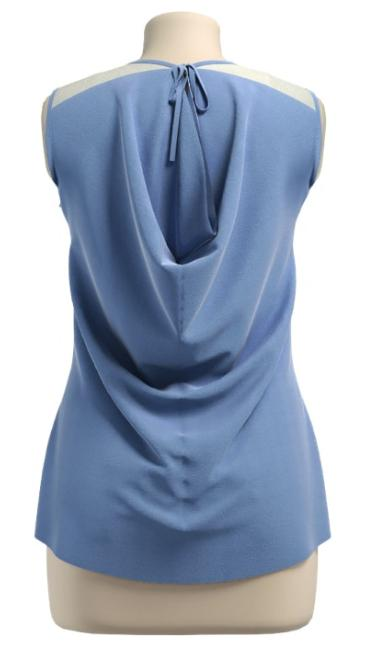
\includegraphics[height=5cm]{img13.jpg}
            \caption{Пример работы программы Clo}
            \label{img:Clo}
        \end{center}
    \end{minipage}
    \hspace{2ex}
    \begin{minipage}[h]{0.4\linewidth}
        \begin{center}
            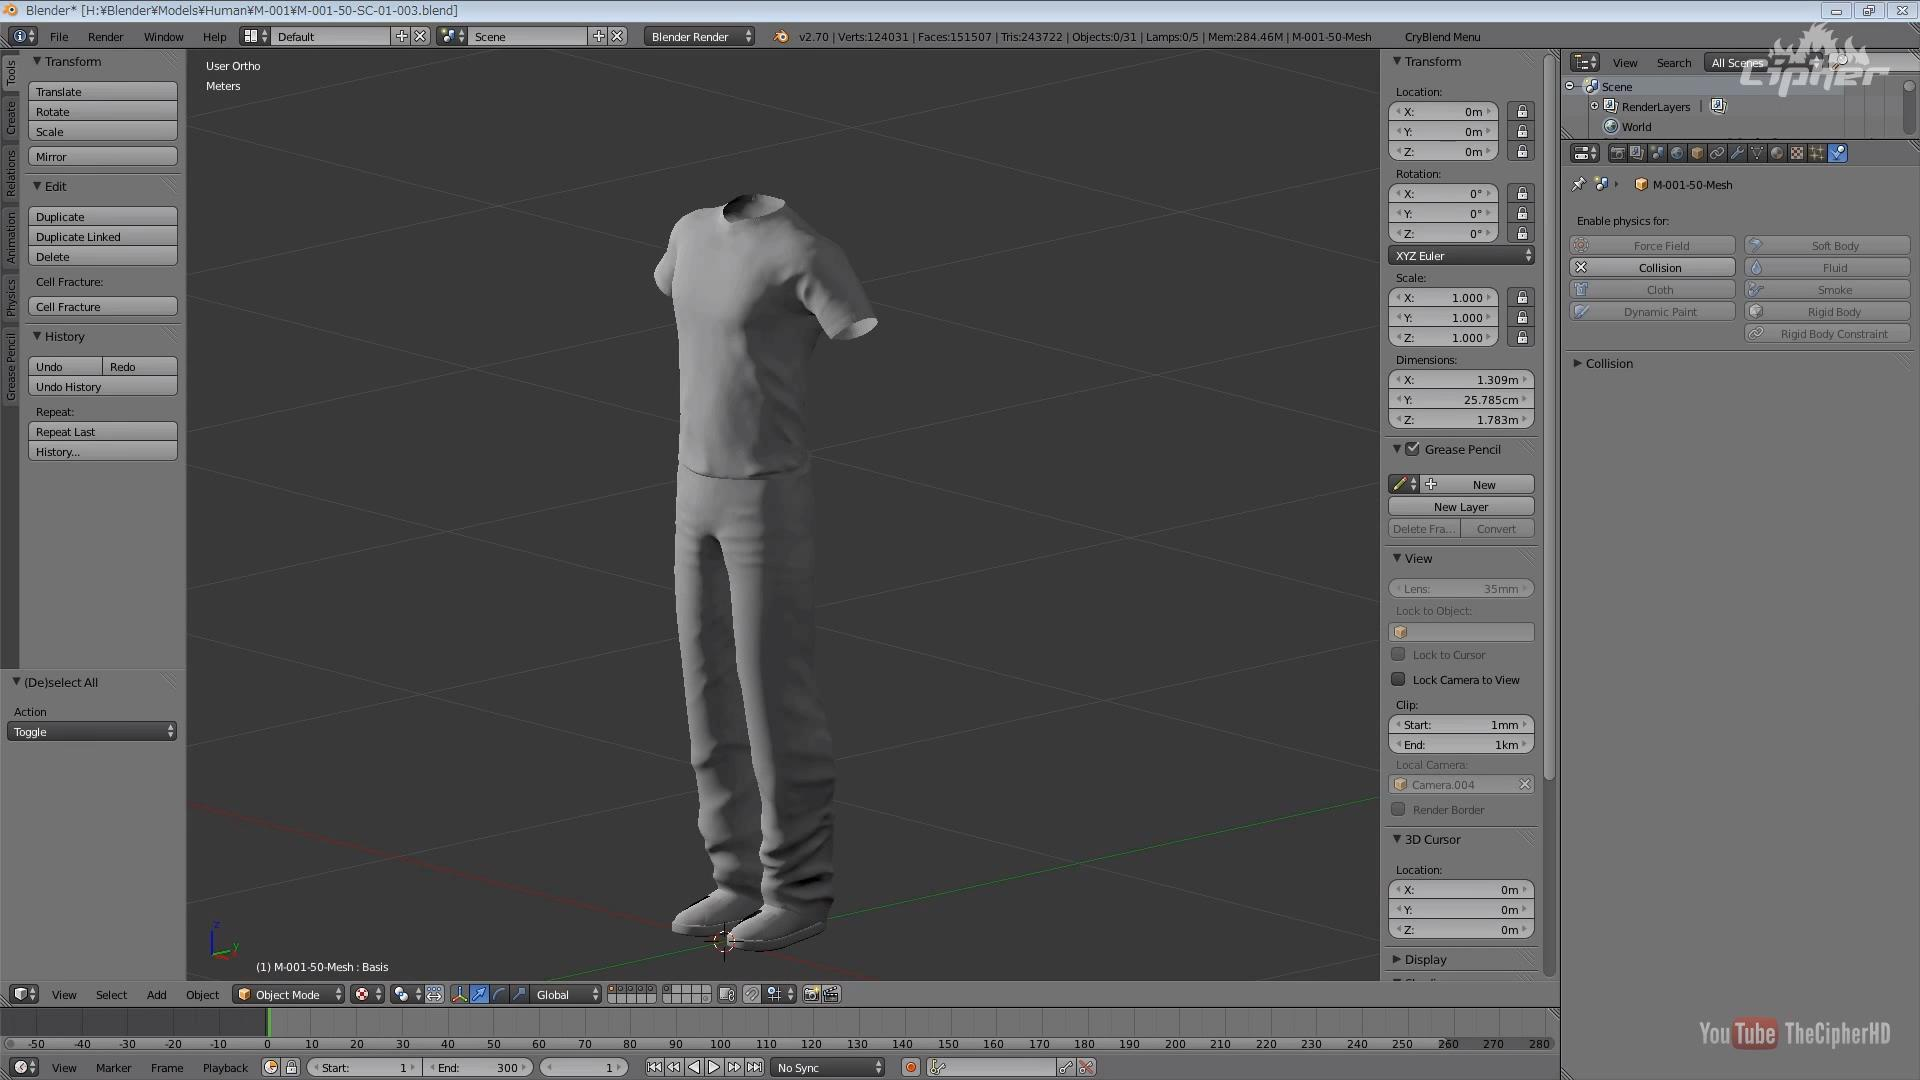
\includegraphics[height=5cm]{img14.jpg}
            \caption{Пример работы программы Browzwear}
            \label{img:Browzwear}
        \end{center}
    \end{minipage}
\end{center}
\end{figure}

Не являются исключением и бесплатные кроссплатформенные приложения для работы с
3D графикой, таких как Blender. Даное приложение предоставляет большой
функционал для моделирования, симуляции, рендеринга, монтажа, записи видео и
создания игр. Дополнения к Blender упрощают моделирование тех, или иных
объектов. В том числе существует дополнение для моделирования ткани и одежды,
пример которого представлен на рисунке \ref{img:blender}.

\img{6cm}{img15.jpg}{Пример визуализации одежды в Blender}{blender}

Также существует аппаратная реализация визуализации одежды PhysiX
Clothing\cite{site03}, пример работы которой представлен на рисунке
\ref{img:physix}.

\img{6cm}{img16.jpg}{Пример визуализации одежды PhysiX Clothing}{physix}

\hyphenation{линий}
\section{Анализ ~алгоритмов ~удаления ~невидимых линий и поверхностей}
\hyphenation{ли-ний}

При выборе алгоритма удаления невидимых линий и поверхностей учитывается
особенность поставленной задачи - работа программы будет выполняться в реальном
режиме при взаимодействии с пользователем. Этот факт предъявляет к алгоритму
требование по скорости работы. Для выбора наиболее подходящего алгоритма
следует рассмотреть уже имеющиеся алгоритмы удаления невидимых линий и
поверхностей.

\subsection{Алгоритм обратной трассировки лучей}
Алгоритм работает в пространстве изображения\cite{raytr}.

Идея: для определения цвета пиксела экрана через него из точки наблюдения
проводится луч, ищется пересечение первым пересекаемым объектом сцены и
определяется освещенность точки пересечения. Эта освещенность складывается из
отраженной и преломленной энергий, полученных от источников света, а также
отраженной и преломленной энергий, идущих от других объектов сцены. После
определения освещенности найденной точки учитывается ослабление света при
прохождении через прозрачный материал и в результате получается цвет точки
экрана.

Плюсы:
\begin{itemize}
    \item изображение, которое строится с учётом явлений дисперсии лучей,
        преломления, а также внутреннего отражения;
    \item возможность использования в параллельных вычислительных системах.
\end{itemize}

Минусы:
\begin{itemize}
    \item трудоёмкие вычисления\cite{tracer_proof};
\end{itemize}

\subsection{Алгоритм, использующий Z-буфер}
Алгоритм работает в пространстве изображения\cite{zbuf}.

Идея: имеется 2 буфера - буфер кадра, который используется для запоминания
цвета каждого пиксела изображения, а также $z$-буфер - отдельный буфер глубины,
используемый для запоминания координаты $z$ (глубины) каждого видимого пиксела
изображения. В процессе работы глубина или значение $z$ каждого нового пиксела,
который нужно занести в буфер кадра, сравнивается с глубиной того пиксела,
который уже занесен в $z$-буфер. Если это сравнение показывает, что новый
пиксел расположен выше пиксела, находящегося в буфере кадра ($z > 0$), то новый
пиксел заносится в цвет рассматриваемого пиксела заносится в буфер кадра, а
координата $z$ - в $z$-буфер. По сути, алгоритм является поиском по $x$ и $y$
наибольшего значения функции $z(x, y)$.

Плюсы:
\begin{itemize}
    \item возможность обработки произвольных поверхностей, аппроксимируемых
        полигонами;
    \item отсутствие требования сортировки объектов по глубине.
\end{itemize}

Минусы:
\begin{itemize}
    \item отсутствие возможности работы с прозрачными и просвечивающими
        объектами (в классической версии).
\end{itemize}

\subsection{Алгоритм Робертса}
Алгоритм работает в объектном пространстве\cite{robert}.

Идея: алгоритм прежде всего удаляет из каждого тела те ребра или грани, которые
экранируются самим телом. Затем каждое из видимых ребер каждого тела
сравнивается с каждым из оставшихся тел для определения того, какая его часть
или части, если таковые есть, экранируются этими телами.

Плюсы:
\begin{itemize}
    \item реализации алгоритма, использующие предварительную приоритетную
        сортировку вдоль оси z и простые габаритные или минимаксные тесты,
        демонстрируют почти линейную зависимость от числа
        объектов\cite{robert}.
\end{itemize}

Минусы:
\begin{itemize}
    \item вычислительная трудоёмкость алгоритма теоретически растет, как
        квадрат числа объектов\cite{robert};
    \item отсутствие возможности работы с прозрачными и просвечивающими
        объектами.
\end{itemize}

\subsection*{Вывод}

Так как главным требованием к алгоритму является скорость работы, алгоритмы
были оценены по следующим критериям:

С учётом результатов в таблице \ref{tab:cmp_del} был выбран алгоритм
\textbf{Z-буфера} удаления невидимых линий и поверхностей.


\section{Анализ методов закрашивания}

Методы закрашивания используются для затенения полигонов (или поверхностей,
аппроксимированных полигонами) в условиях некоторой сцены, имеющей источники
освещения. С учётом взаимного положения рассматриваемого полигона и источника
света находится уровень освещенности по закону Ламберта (\ref{for:lambert}):
\begin{equation}
    \label{for:lambert}
    I_{\alpha} = I_0 \cdot \cos{(\alpha)}
\end{equation}

где $I_{\alpha}$ - уровень освёщенности в рассматриваемой точке, $I_0$ -
максимальный уровень освёщенности, а $\alpha$ - угол между вектором нормали к
плоскости и вектором, направленным от рассматриваемой точки к источнику
освещения (в случае нормированных векторов может быть рассчитан как скалярное
произведение данных векторов).

\subsection{Простая закраска}

Идея: вся грань закрашивается одним уровнем интенсивности, который зависит
высчитывается по закону Ламберта\cite{rogers}. При данной закраске все
плоскости (в том числе и те, что аппроксимируют фигуры вращения), будут
закрашены однотонно, что в случае с фигурами вращения будет давать ложные
ребра.

Плюсы:
\begin{itemize}
    \item используется для работы с многогранниками, обладающими преимущественно диффузным отражением.
\end{itemize}

Минусы:

\begin{itemize}
    \item плохо подходит для фигур вращения: видны ребра.
\end{itemize}

\subsection{Закраска по Гуро}
Идея: билинейная интерполяция в каждой точке интенсивности освещения в вершинах\cite{lmodels}.

Нормаль к вершине можно найти несколькими способами:
\begin{itemize}
    \item интерполировать нормали прилегающих к вершине граней;
    \item использовать геометрические свойства фигуры (так, например, в случае
        со сферой ненормированный вектор нормали будет в точности
        соответствовать вектору от центра сферы до рассматриваемой точки).
\end{itemize}

После нахождения нормали ко всем вершинам находится интенсивность в каждой
вершине по закону Ламберта (\ref{for:lambert}).  Затем алгоритм проходится
сканирующими строками по рассматриваемому полигону для всех $y: y \in [y_{min};
y_{max}]$. Каждая сканирующая строка пересекает 2 ребра многоугольника, пусть
для определённости это будут ребра через одноименные вершины: $MN$ и $KL$. В
точках пересечения высчитывается интенсивность путём интерполяции интенсивности
в вершинах. Так, для точки пересечения с ребром $MN$ интенсивность будет
рассчитана как (\ref{for:int_mn}):
\begin{equation}
    \label{for:int_mn}
    I_{MN} = \frac{l_1}{l_0} \cdot I_M + \frac{l_2}{l_0} \cdot I_N
\end{equation}
где $l_1$ - расстояние от точки пересечения до вершины $N$, $l_2$ - расстояние
от точки пересечения до вершины $M$, $l_0$ - длина ребра $MN$.  Для точки
пересечения сканирующей строки с ребром $KL$ интенсивность высчитывается
аналогично.

Далее, после нахождения точек пересечения, алгоритм двигается по $Ox$ от левой
точки пересечения $X_{left}$ до правой точки пересечения $X_{right}$ и в каждой
точке $\mathcal{X}$ интенсивность рассчитывается как (\ref{for:int_x}):
\begin{equation}
    \label{for:int_x}
    I_{\mathcal{X}} = \frac{\mathcal{X} - X_{left}}{X_{right} - X_{left}} \cdot
    I_{X_{right}} + \frac{X_{right} - \mathcal{X}}{X_{right} - X_{left}} \cdot
    I_{X_{left}}
\end{equation}

Плюсы:
\begin{itemize}
    \item преимущественно используется с фигурами вращения с диффузным
        отражением, аппроксимированными полигонами.
\end{itemize}

Минусы:
\begin{itemize}
    \item при закраске многогранников ребра могут стать незаметными.
\end{itemize}

\subsection{Закраска по Фонгу}
Идея: данный алгоритм работает похожим на алгоритм Гуро образом, однако
ключевым отличием является то, что интерполируются не интенсивности в вершинах,
а нормали\cite{lmodels}. Таким образом, закон Ламберта в данном алгоритме
применяется в каждой точке, а не только в вершинах, что делает этот алгоритм
гораздо более трудоёмким, однако с его помощью можно гораздо лучше изображаются
блики.

Плюсы:
\begin{itemize}
    \item преимущественно используется с фигурами вращения с зеркальным
        отражением, аппроксимированными полигонами.
\end{itemize}

Минусы:
\begin{itemize}
    \item самый трудоёмкий алгоритм из рассмотренных\cite{rogers}.
\end{itemize}

\subsection*{Вывод}

 Так как требованиями к алгоритму являются высокая скорость работы, а также
 возможность закраски фигур вращения с диффузными свойствами отражения,
 алгоритмы были оценены по следующим критериям: С учётом результатов в таблице
 \ref{tab:cmp_paint} был выбран алгоритм закраски \textbf{Гуро}.
